%%\documentclass[a4paper,12pt,oneside]{llncs}
\documentclass[12pt,letterpaper]{article}
\usepackage[right=2cm,left=3cm,top=2cm,bottom=2cm,headsep=0cm]{geometry}

%%%%%%%%%%%%%%%%%%%%%%%%%%%%%%%%%%%%%%%%%%%%%%%%%%%%%%%%%%%
%% Juego de caracteres usado en el archivo fuente: UTF-8
\usepackage{ucs}
\usepackage[utf8x]{inputenc}

%%%%%%%%%%%%%%%%%%%%%%%%%%%%%%%%%%%%%%%%%%%%%%%%%%%%%%%%%%%
%% Juego de caracteres usado en la salida dvi
%% Otra posibilidad: \usepackage{t1enc}
\usepackage[T1]{fontenc}

%%%%%%%%%%%%%%%%%%%%%%%%%%%%%%%%%%%%%%%%%%%%%%%%%%%%%%%%%%%
%% Ajusta maergenes para a4
%\usepackage{a4wide}

%%%%%%%%%%%%%%%%%%%%%%%%%%%%%%%%%%%%%%%%%%%%%%%%%%%%%%%%%%%
%% Uso fuente postscript times, para que los ps y pdf queden y pequeños...
\usepackage{times}

%%%%%%%%%%%%%%%%%%%%%%%%%%%%%%%%%%%%%%%%%%%%%%%%%%%%%%%%%%%
%% Posibilidad de hipertexto (especialmente en pdf)
%\usepackage{hyperref}
\usepackage[bookmarks = true, colorlinks=true, linkcolor = black, citecolor = black, menucolor = black, urlcolor = black]{hyperref}

%%%%%%%%%%%%%%%%%%%%%%%%%%%%%%%%%%%%%%%%%%%%%%%%%%%%%%%%%%%
%% Graficos 
\usepackage{graphics,graphicx}

%%%%%%%%%%%%%%%%%%%%%%%%%%%%%%%%%%%%%%%%%%%%%%%%%%%%%%%%%%%
%% Ciertos caracteres "raros"...
\usepackage{latexsym}

%%%%%%%%%%%%%%%%%%%%%%%%%%%%%%%%%%%%%%%%%%%%%%%%%%%%%%%%%%%
%% Matematicas aun más fuertes (american math dociety)
\usepackage{amsmath}

%%%%%%%%%%%%%%%%%%%%%%%%%%%%%%%%%%%%%%%%%%%%%%%%%%%%%%%%%%%
\usepackage{multirow} % para las tablas
\usepackage[spanish,es-tabla]{babel}

%%%%%%%%%%%%%%%%%%%%%%%%%%%%%%%%%%%%%%%%%%%%%%%%%%%%%%%%%%%
%% Fuentes matematicas lo mas compatibles posibles con postscript (times)
%% (Esto no funciona para todos los simbolos pero reduce mucho el tamaño del
%% pdf si hay muchas matamaticas....
\usepackage{mathptm}
\usepackage{xcolor}

%%% VARIOS:
%\usepackage{slashbox}
\usepackage{verbatim}
\usepackage{array}
\usepackage{listings}
\usepackage{multirow}

%% MARCA DE AGUA
%% Este package de "draft copy" NO funciona con pdflatex
%%\usepackage{draftcopy}
%% Este package de "draft copy" SI funciona con pdflatex
%%%\usepackage{pdfdraftcopy}
%%%%%%%%%%%%%%%%%%%%%%%%%%%%%%%%%%%%%%%%%%%%%%%%%%%%%%%%%%%
%% Indenteacion en español...
\usepackage[spanish]{babel}

\usepackage{listingsutf8}
% Para escribir código en C
% \begin{lstlisting}[language=C]
% #include <stdio.h>
% int main(int argc, char* argv[]) {
% puts("Hola mundo!");
% }
% \end{lstlisting}


\title{Comunicación y tratado de ficheros secuencial}
\author{Jesús Rodríguez Heras}

\begin{document}
	
	\maketitle
	\begin{abstract} %Poner esto en todas las prácticas de PCTR
		\begin{center}
			En este documento se desarrolla un tutorial de envío y recepción de ficheros mediante SSH entre los dispositivos del proyecto de manera secuencial y automática.
			
			Para conseguir dicha finalidad, las tarjetas iniciarán automáticamente un proceso que comprobará si les envían un fichero nuevo y, en caso de que así sea, trabajarán con el y lo enviarán a la siguiente tarjeta, o, en caso de que no esté conectada, al ordenador central.
			
			El fichero será recibido en el directorio \texttt{\textasciitilde/ficheros/recibir} e irá pasando por los directorios \texttt{\textasciitilde/ficheros/desencriptar}, \texttt{\textasciitilde/ficheros/trabajar} y \texttt{\textasciitilde/ficheros/enviar} antes de ser enviado al siguiente dispositivo.
		\end{center}
	\end{abstract}
	\thispagestyle{empty}
	\newpage
	
	\tableofcontents
	\newpage
	
	%%\listoftables
	%%\newpage
	
	%%\listoffigures
	%%\newpage
	
	%%%% REAL WORK BEGINS HERE:
	
	%%Configuracion del paquete listings
	\lstset{language=bash, numbers=left, numberstyle=\tiny, numbersep=10pt, firstnumber=1, stepnumber=1, basicstyle=\small\ttfamily, tabsize=2, extendedchars=true, inputencoding=utf8/latin1, breaklines=true}
	

\section{Introducción}
Para realizar una comunicación automática y secuencial entre los distintos dispositivos, cada tarjeta Zybo Zynq 7010 contará con la siguiente estructura de directorios:\\

%Los que están comentados es porque ésta es la versión que emula el trabajo de Cristian, descomentarla para ver el proceso completo sin la emulación del trabajo de Cristian.
\texttt{
\textasciitilde/ficheros/backups/\\
%\textcolor{white}{.}\hspace{3.15cm}|\hspace{1.8cm}|ViejoDesencriptar.txt\\
\textcolor{white}{.}\hspace{3.15cm}|\hspace{1.8cm}|ViejoEnviar.txt\\
\textcolor{white}{.}\hspace{3.15cm}|\hspace{1.8cm}|ViejoRecibir.txt\\
\textcolor{white}{.}\hspace{3.15cm}|\hspace{1.8cm}|ViejoTrabajar.txt\\
\textcolor{white}{.}\hspace{3.15cm}|desencriptar/..\\
\textcolor{white}{.}\hspace{3.15cm}|enviar/..\\
\textcolor{white}{.}\hspace{3.15cm}|recibir/..\\
\textcolor{white}{.}\hspace{3.15cm}|trabajar/..\\
\textcolor{white}{.}\hspace{3.15cm}|Automatico.sh\\
\textcolor{white}{.}\hspace{3.15cm}|Borrar.sh\\
\textcolor{white}{.}\hspace{3.15cm}|Cristian.sh\\
%\textcolor{white}{.}\hspace{3.15cm}|Desencriptando.sh\\
\textcolor{white}{.}\hspace{3.15cm}|Enviando.sh\\
\textcolor{white}{.}\hspace{3.15cm}|Recibiendo.sh\\
%\textcolor{white}{.}\hspace{3.15cm}|Tabajando.sh
}

Este árbol de directorios estará en el archivo \texttt{ficheros.tar.gz} que se encontrará en el ordenador central y será distribuido a cada tarjeta mediante ssh\footnote{Recordemos que, tanto para \texttt{ssh} como para \texttt{scp}, el elemento \texttt{zyboX} es el identificador de la tarjeta Zybo con la que estamos trabajando.} con el siguiente comando:
\begin{center}
	\texttt{sshpass -p zyboX scp -o StrictHostKeyChecking=no ficheros.tar.gz zyboX@zyboX:}
\end{center}

Luego, entramos en la tarjeta mediante ssh con el siguiente comando:
\begin{center}
	\texttt{sshpass -p zyboX ssh -o StrictHostKeyChecking=no zyboX@zuboX}
\end{center}

Para ver si tenemos el archivo \texttt{ficheros.tar.gz} usamos el comando:
\begin{center}
	\texttt{ls}
\end{center}

%\begin{figure}[h]
%	\centering
%	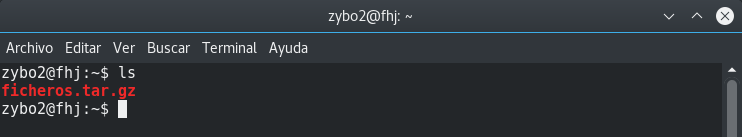
\includegraphics[scale=0.6]{ls.png}
%	\caption{Salida del comando ls.}
%	\label{Salida del comando ls}
%\end{figure}

A continuación, aplicamos el siguiente comando para descomprimir el archivo \texttt{ficheros.tar.gz}:
\begin{center}
	\texttt{tar -xzvf ficheros.tar.gz}
\end{center}

Se nos creará el árbol de directorios anteriormente citado en el directorio \texttt{/home} de la tarjeta Zybo a la que hayamos accedido.
% tal como podemos ver en la siguiente imagen:
%\begin{figure}[h]
%	\centering
%	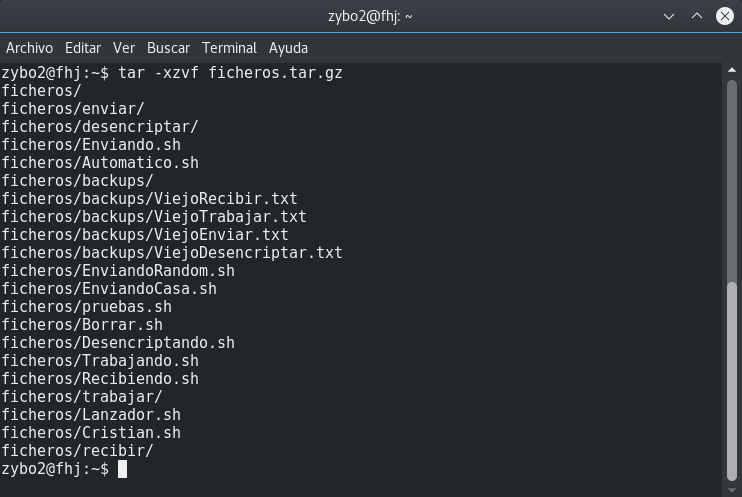
\includegraphics[scale=0.5]{arbol.png}
%	\caption{Descompresión del archivo \texttt{ficheros.tar.gz}.}
%	\label{Descompresión del archivo ficheros.tar.gz}
%\end{figure}

Para que la automatización del proceso se lleve a cabo correctamente, también tendremos que modificar el fichero \texttt{/etc/hosts} de la tarjeta. Para ello, enviamos el fichero con el siguiente comando:
\begin{center}
	\texttt{sshpass -p zyboX scp -o StrictHostKeyChecking=no hosts zyboX@zyboX:}
\end{center}

Y, luego, lo copiamos como super-usuario\footnote{Comando: \texttt{su}, y contraseña \texttt{root}.} en el directorio \texttt{/etc} con el siguiente comando:
\begin{center}
	\texttt{cp hosts /etc}
\end{center}

Una vez hecho esto, el proceso de automatización estaría listo para ser lanzado.

\section{Directorios}
En este apartado, describiremos los distintos directorios que podemos encontrar en las tarjetas Zybo una vez que se ha descomprimido el archivo \texttt{ficheros.tar.gz}.

Dicha descripción se hará siguiendo el orden que recorrerá el archivo recibido desde el ordenador central, salvo el directorio \texttt{/backups} que se describirá primero ya que no interviene de forma directa en el camino a recorrer por el archivo recibido.

\subsection{Directorio \texttt{/backups}}
En este directorio se guardarán los estados de los siguientes directorios generados por el comando \texttt{stat}\footnote{Para más información leer el manual del comando \texttt{stat} en este \href{https://linux.die.net/man/2/stat}{\textcolor{blue}{enlace}}.}.
\begin{itemize}
	\item \textbf{\texttt{ViejoDesencriptar.txt}:} Este fichero contendrá el estado del directorio \texttt{/desencriptar} una vez que el script \texttt{Desencriptando.sh} lo compruebe. Si no se producen cambios en dicho directorio, este fichero no se modificará.
	\item \textbf{\texttt{ViejoEnviar.txt}:} Este fichero contendrá el estado del directorio \texttt{/enviar} una vez que el script \texttt{Enviando.sh} lo compruebe. Si no se producen cambios en dicho directorio, este fichero no se modificará.
	\item \textbf{\texttt{ViejoRecibir.txt}:} Este fichero contendrá el estado del directorio \texttt{/recibir} una vez que el script \texttt{Recibiendo.sh} lo compruebe. Si no se producen cambios en dicho directorio, este fichero no se modificará.
	\item \textbf{\texttt{ViejoTrabajar.txt}:} Este fichero contendrá el estado del directorio \texttt{/trabajar} una vez que el script \texttt{Trabajando.sh} lo compruebe. Si no se producen cambios en dicho directorio, este fichero no se modificará.
\end{itemize}

\subsection{Directorio \texttt{/recibir}}
Este directorio contendrá los ficheros enviados por el ordenador central mediante ssh\footnote{Para ver como enviar ficheros desde el ordenador central hasta este directorio, ver el documento ``Envío y recepción de ficheros con sshpass''.}.

Tendremos un script en segundo plano, \texttt{Recibiendo.sh}, que comprobará si hay algún cambio en el directorio. Si lo hay\footnote{Si hay un cambio en el directorio, supone que ha llegado un nuevo archivo por parte del ordenador.}, envía el archivo al directorio \texttt{/desencriptar}.

\subsection{Directorio \texttt{/desencriptar}}
Este directorio contendrá los ficheros enviados desde el directorio \texttt{/recibir} por el script \texttt{Recibiendo.sh} que comprobará el estado del directorio anterior.

Tendremos un script en segundo plano, \texttt{Cristian.sh} que comprobará si hay algún cambio en el directorio. Si lo hay, envía el archivo al directorio \texttt{/trabajar}.

\subsection{Directorio \texttt{/trabajar}}
Este directorio contendrá los ficheros enviados por el script \texttt{Cristian.sh} que comprobará el estado del directorio anterior.

Aquí, será también el script \texttt{Cristian.sh} el que tome partido, ya que para simular un tratamiento de datos, es este script el que añade al archivo una nueva línea diciendo que el archivo (inicialmente enviado por el ordenador central) ha sido tratado en la tarjeta en la que nos encontremos.

Concretamente, la línea que introduce en el archivo es la siguiente:
\begin{center}
	\texttt{Archivo tratado en zyboX}
\end{center}

Siendo zyboX el identificador de la tarjeta con la que estamos trabajando.

\subsection{Directorio \texttt{/enviar}}
Este directorio contendrá los ficheros enviados por el script \texttt{Cristian.sh} que comprobará el estado del directorio anterior.

Aquí también tendremos un script en segundo plano, \texttt{Enviando.sh}, que comprobará si hay algún cambio en los ficheros y los enviará al siguiente dispositivo mediante ssh\footnote{Para ver como funciona el envío de ficheros mediante ssh, ver el documento ``Envío y recepcion de ficheros con sshpass''.}.


\section{Scripts}
En este apartado, describiremos los distintos scripts que podemos encontrar en las tarjetas Zybo con su descripción y código correspondiente.

Dicha descripción se hará siguiendo el orden que recorrerá el archivo recibido desde el ordenador central hasta ser enviado al siguiente dispositivo.

Para comprobar el estado de todos los directorios, usaremos el comando \texttt{stat} para comprobar el estado de los directorios.

En el trabajo aquí mencionado se emula el desencriptado de un fichero, adición de información, cifrado, y envío del mismo a otro dispositivo\footnote{Para cambiar dicho comportamiento, solo tendremos que modificar los scritps que se encargan de automatizar el proceso.}.

%Debemos tener en cuenta que, para emular el trabajo de nuestro compañero Cristian, hemos hecho que el script \texttt{Cristian.sh} sea el que ``desencripta'' el fichero, añade información y ``encripta'' el fichero de nuevo, justo antes de enviarlo al directorio \texttt{/enviar}.

\subsection{\texttt{Lanzador.sh}}
Este script se encarga de lanzar el script \texttt{Automatico.sh} mediante la herramienta cron\footnote{Para más información, ver el manual de crontab en este \href{https://linux.die.net/man/5/crontab}{\textcolor{blue}{enlace}}.} al inicio del sistema operativo Xillinux.

Para usarlo, debemos usar el siguiente comando:
\begin{center}
	\texttt{crontab -e}
\end{center}

Y, luego, añadir la regla que queramos que se ejecute al final del fichero. En nuestro caso es la siguiente:
\begin{center}
	\texttt{@reboot (cd \textasciitilde/ficheros; ./Lanzador.sh)}
\end{center}

Esto hará que la herramienta cron inicie este script al iniciar el sistema operativo Xillinux de las tarjetas.
\subsubsection{Código}
\lstinputlisting[language=Bash]{Scripts/Lanzador.sh}
\begin{center}
	Código de \texttt{Lanzador.sh}.
\end{center}

\newpage
\subsubsection{Diagrama de flujo}
\begin{figure}[h]
	\centering
	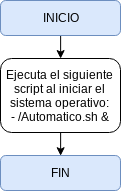
\includegraphics[scale=0.9]{Diagramas/Lanzador.png}
	\caption{Diagrama de flujo de \texttt{Lanzador.sh}.}
	\label{Diagrama de flujo de Lanzador.sh}
\end{figure}

\subsection{\texttt{Automatico.sh}}
Este script es el encargado de lanzar el resto de scripts cada segundo para que vayan comprobando los directorios correspondientes y se produzca la comunicación de forma automática.

\subsubsection{Código}
\lstinputlisting[language=Bash]{Scripts/Automatico.sh}
\begin{center}
	Código de \texttt{Automatico.sh}.
\end{center}

\newpage
\subsubsection{Diagrama de flujo}
\begin{figure}[h]
	\centering
	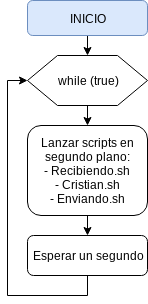
\includegraphics[scale=0.9]{Diagramas/Automatico.png}
	\caption{Diagrama de flujo de \texttt{Automatico.sh}.}
	\label{Diagrama de flujo de Automatico.sh}
\end{figure}

\subsection{\texttt{Recibiendo.sh}}
Este script es el encargado de comprobar periódicamente el estado del directorio \texttt{/recibir} y, si llega un archivo nuevo, enviarlo al directorio \texttt{/desencriptar}.

\subsubsection{Código}
\lstinputlisting[language=Bash]{Scripts/Recibiendo.sh}
\begin{center}
	Código de \texttt{Recibiendo.sh}.
\end{center}

\newpage
\subsubsection{Diagrama de flujo}
\begin{figure}[h]
	\centering
	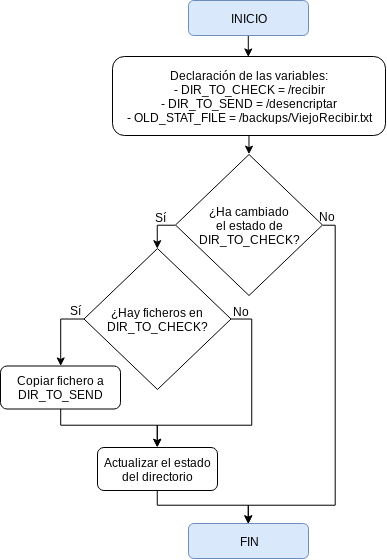
\includegraphics[scale=0.8]{Diagramas/Recibiendo.png}
	\caption{Diagrama de flujo de \texttt{Recibiendo.sh}.}
	\label{Diagrama de flujo de Recibiendo.sh}
\end{figure}

\newpage
\subsection{\texttt{Cristian.sh}}
Este script es el encargado de emular el trabajo de nuestro compañero Cristian. Se encarga de comprobar periódicamente el estado del directorio \texttt{/desencriptar}, mueve el archivo allí situado al directorio \texttt{/trabajar} (simulando el desencriptado) y allí le añade un texto tal como el siguiente:
\begin{center}
	\texttt{Archivo tratado en zyboX}
\end{center}

Siendo zyboX el identificador de la tarjeta con la que estamos trabajando.

Por último, envía el fichero al directorio \texttt{/enviar}.

\subsubsection{Código}
\lstinputlisting[language=Bash]{Scripts/Cristian.sh}
\begin{center}
	Código de \texttt{Cristian.sh}.
\end{center}

\subsubsection{Diagrama de flujo}
\begin{figure}[h]
	\centering
	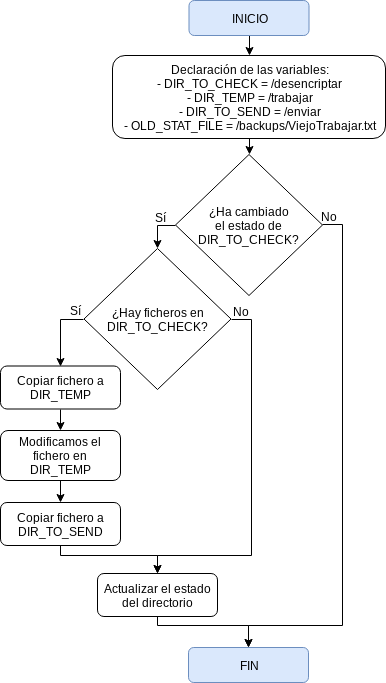
\includegraphics[scale=0.7]{Diagramas/Cristian.png}
	\caption{Diagrama de flujo de \texttt{Cristian.sh}.}
	\label{Diagrama de flujo de Cristian.sh}
\end{figure}

\newpage
\subsection{\texttt{Enviando.sh}}
Este script es el encargado de comprobar periódicamente el estado del directorio \texttt{/enviar} y, cuando detecta un cambio, envía el archivo a la siguiente tarjeta, o, si ésta se encuentra desconectada, al ordenador central.

A la hora de comprobar si la siguiente tarjeta está conectada o no, se hace enviando un comando ping a la siguiente tarjeta.

Para que podamos usar el comando ping desde este script, debemos darle permisos de ejecución en modo usuario de la siguiente forma:
\begin{enumerate}
	\item Entramos como super-usuario con el comando \texttt{su} y contraseña \texttt{zyboX} (siendo X el identificador de la tarjeta con la que estamos trabajando).
	\item A continuación, introducimos el siguiente comando:
	\begin{center}
		\texttt{chmod u+s /bin/ping}
	\end{center}
	Y con eso, quedaría activado el comando \texttt{ping} para poder usarlo desde este script.
\end{enumerate}

\subsubsection{Código}
\lstinputlisting[language=Bash]{Scripts/Enviando.sh}
\begin{center}
	Código de \texttt{Enviando.sh}.
\end{center}

\newpage
\subsubsection{Diagrama de flujo}
\begin{figure}[h]
	\centering
	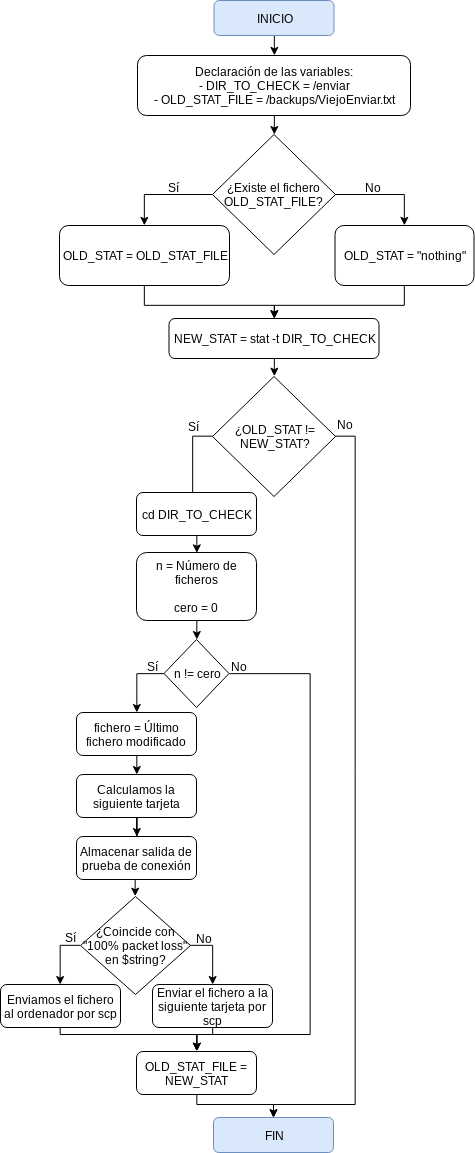
\includegraphics[scale=0.65]{Diagramas/Enviando.png}
	\caption{Diagrama de flujo de \texttt{Diagramas/Enviando.sh}.}
	\label{Diagrama de flujo de Enviando.sh}
\end{figure}


\subsection{\texttt{Borrar.sh}}
Este script se encarga de vaciar los directorios \texttt{recibir}, \texttt{desencriptar}, \texttt{trabajar} y \texttt{recibir} de las tarjetas Zybo.

Para ejecutarlo solo debemos usar el siguiente comando en el directorio \texttt{/ficheros} de las tarjetas Zybo:
\begin{center}
	\texttt{./Borrar.sh}
\end{center}

\subsubsection{Código}
\lstinputlisting[language=Bash]{Scripts/Borrar.sh}
\begin{center}
	Código de \texttt{Borrar.sh}.
\end{center}

\subsubsection{Diagrama de flujo}
\begin{figure}[h]
	\centering
	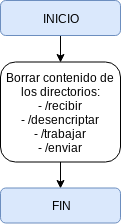
\includegraphics[scale=0.9]{Diagramas/Borrar.png}
	\caption{Diagrama de flujo de \texttt{Borrar.sh}.}
	\label{Diagrama de flujo de Borrar.sh}
\end{figure}



%\subsection{\texttt{Desencriptando.sh}}

%\subsection{\texttt{Trabajando.sh}}

\end{document}